\chapter{Paging}

\section{Motivation for Paging}

Paging is a memory management technique that eliminates the need for contiguous physical memory allocation.

Problems with contiguous allocation:

\begin{itemize}
\item External fragmentation
\item Difficult memory allocation
\item Process growth limitations
\item Inefficient memory utilization
\end{itemize}

Paging solves these problems by dividing memory into fixed-size blocks.

\begin{figure}[H]
\centering
\begin{tikzpicture}
\draw (0,0) rectangle (2,6);
\node at (1,5.5) {Free};
\node at (1,4.5) {P1};
\node at (1,3.5) {Free};
\node at (1,2.5) {P2};
\node at (1,1.5) {Free};
\node at (1,0.5) {P3};

\draw (0,5)--(2,5);
\draw (0,4)--(2,4);
\draw (0,3)--(2,3);
\draw (0,2)--(2,2);
\draw (0,1)--(2,1);

\node at (5,3) {External Fragmentation};
\end{tikzpicture}
\caption{Fragmentation in Contiguous Allocation}
\end{figure}

\section{Paging Fundamentals}

Paging divides:

\begin{itemize}
\item Logical memory into pages
\item Physical memory into frames
\end{itemize}

Page size equals frame size.

\[
\text{Page Size} = \text{Frame Size}
\]

Common page sizes:

\begin{itemize}
\item 4 KB
\item 8 KB
\item 16 KB
\item 2 MB (Huge Page)
\item 1 GB (Huge Page)
\end{itemize}

\section{Pages and Frames}

\subsection{Pages}

Fixed-size logical memory blocks.

\subsection{Frames}

Fixed-size physical memory blocks.

\begin{figure}[H]
\centering
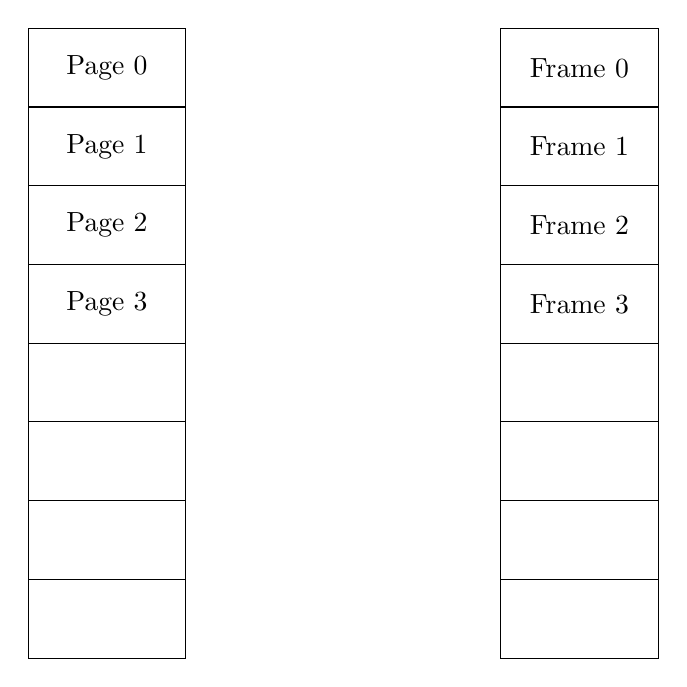
\begin{tikzpicture}

\draw (0,0) rectangle (2,8);

\foreach \y in {1,2,3,4,5,6,7}
{
\draw (0,\y)--(2,\y);
}

\node at (1,7.5) {Page 0};
\node at (1,6.5) {Page 1};
\node at (1,5.5) {Page 2};
\node at (1,4.5) {Page 3};

\draw (6,0) rectangle (8,8);

\foreach \y in {1,2,3,4,5,6,7}
{
\draw (6,\y)--(8,\y);
}

\node at (7,7.5) {Frame 0};
\node at (7,6.5) {Frame 1};
\node at (7,5.5) {Frame 2};
\node at (7,4.5) {Frame 3};

\end{tikzpicture}
\caption{Pages and Frames}
\end{figure}

\section{Logical Address Structure}

Logical address consists of:

\[
\text{Logical Address} =
\langle Page\ Number,\ Offset \rangle
\]

Example:

\[
16\text{-bit Address}
\]

Page Size:

\[
1KB = 2^{10}
\]

Offset bits:

\[
10
\]

Page Number bits:

\[
16-10 = 6
\]

Logical Address:

\[
\langle p,d \rangle
\]

\section{Physical Address Structure}

Physical address consists of:

\[
\langle Frame\ Number,\ Offset \rangle
\]

\begin{figure}[H]
\centering
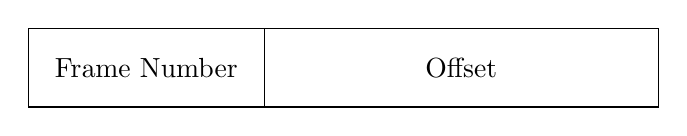
\begin{tikzpicture}

\draw (0,0) rectangle (8,1);

\draw (3,0)--(3,1);

\node at (1.5,0.5) {Frame Number};

\node at (5.5,0.5) {Offset};

\end{tikzpicture}
\caption{Physical Address Format}
\end{figure}

\section{Address Translation}

Address translation converts logical addresses into physical addresses.

\subsection{Example}

Logical Address:

\[
(5,100)
\]

Page Table:

\[
Page\ 5 \rightarrow Frame\ 12
\]

Physical Address:

\[
(12,100)
\]

\begin{figure}[H]
\centering
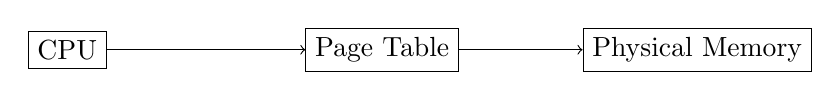
\begin{tikzpicture}

\node[draw] (cpu) at (0,0) {CPU};

\node[draw] (pt) at (4,0) {Page Table};

\node[draw] (mem) at (8,0) {Physical Memory};

\draw[->] (cpu)--(pt);
\draw[->] (pt)--(mem);

\end{tikzpicture}
\caption{Address Translation Process}
\end{figure}

\section{Page Tables}

A page table maps pages to frames.

\subsection{Example}

\begin{center}
\begin{tabular}{cc}
\toprule
Page & Frame \\
\midrule
0 & 5 \\
1 & 2 \\
2 & 8 \\
3 & 9 \\
4 & 1 \\
5 & 12 \\
\bottomrule
\end{tabular}
\end{center}

\subsection{Purpose}

\begin{itemize}
\item Address translation
\item Memory protection
\item Page tracking
\end{itemize}

\section{Page Table Entries}

Typical Page Table Entry (PTE):

\begin{center}
\begin{tabular}{ll}
\toprule
Field & Purpose \\
\midrule
Frame Number & Physical Frame \\
Valid Bit & Page Present? \\
Protection Bits & Access Rights \\
Dirty Bit & Modified Page \\
Reference Bit & Recently Used \\
\bottomrule
\end{tabular}
\end{center}

\section{Translation Lookaside Buffer (TLB)}

TLB is a special hardware cache storing recent page table entries.

\subsection{Motivation}

Without TLB:

\begin{enumerate}
\item Access page table
\item Access memory
\end{enumerate}

Two memory accesses required.

With TLB:

\begin{enumerate}
\item Check TLB
\item Access memory
\end{enumerate}

One memory access on hit.

\begin{figure}[H]
\centering
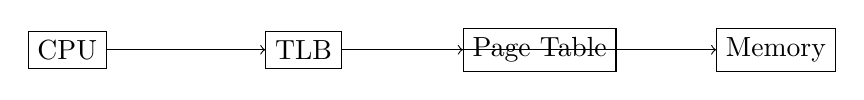
\begin{tikzpicture}

\node[draw] (cpu) at (0,0) {CPU};

\node[draw] (tlb) at (3,0) {TLB};

\node[draw] (pt) at (6,0) {Page Table};

\node[draw] (mem) at (9,0) {Memory};

\draw[->] (cpu)--(tlb);
\draw[->] (tlb)--(mem);
\draw[->] (tlb)--(pt);

\end{tikzpicture}
\caption{TLB-Based Translation}
\end{figure}

\section{Effective Memory Access Time}

\subsection{Formula}

Let:

\[
h = TLB\ hit\ ratio
\]

\[
t = TLB\ lookup\ time
\]

\[
m = Memory\ access\ time
\]

Then:

\[
EMAT = h(t+m)+(1-h)(t+2m)
\]

\subsection{Numerical Example}

Given:

\[
t=10ns
\]

\[
m=100ns
\]

\[
h=0.95
\]

Calculation:

\[
EMAT =
0.95(10+100)+0.05(10+200)
\]

\[
EMAT =
104.5+10.5
\]

\[
EMAT = 115ns
\]

\section{Hierarchical Paging}

Large address spaces require huge page tables.

Solution:

Multi-level hierarchy.

\begin{figure}[H]
\centering
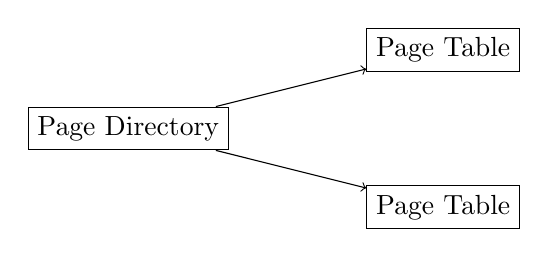
\begin{tikzpicture}

\node[draw] (d) at (0,0) {Page Directory};

\node[draw] (p1) at (4,1) {Page Table};

\node[draw] (p2) at (4,-1) {Page Table};

\draw[->] (d)--(p1);
\draw[->] (d)--(p2);

\end{tikzpicture}
\caption{Hierarchical Paging}
\end{figure}

\section{Multilevel Paging}

Modern systems use multiple levels.

Example:

32-bit system:

\begin{itemize}
\item Page Directory
\item Page Table
\item Offset
\end{itemize}

64-bit systems may use:

\begin{itemize}
\item 4-level paging
\item 5-level paging
\end{itemize}

Example:

\[
48-bit\ Virtual\ Address
\]

\[
9+9+9+9+12
\]

\section{Inverted Page Tables}

Instead of one entry per page:

One entry per frame.

\subsection{Advantages}

\begin{itemize}
\item Smaller memory overhead
\item Suitable for large address spaces
\end{itemize}

\subsection{Disadvantages}

\begin{itemize}
\item Slower lookup
\item Requires hashing
\end{itemize}

\section{Hashed Page Tables}

Used for very large virtual address spaces.

Hash Function:

\[
Hash(VPN)
\]

VPN:

Virtual Page Number.

\begin{figure}[H]
\centering
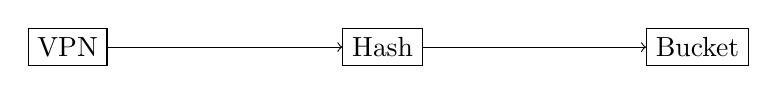
\begin{tikzpicture}

\node[draw] (vpn) at (0,0) {VPN};

\node[draw] (hash) at (4,0) {Hash};

\node[draw] (bucket) at (8,0) {Bucket};

\draw[->] (vpn)--(hash);
\draw[->] (hash)--(bucket);

\end{tikzpicture}
\caption{Hashed Page Table}
\end{figure}

\section{Shared Pages}

Multiple processes may share pages.

Common examples:

\begin{itemize}
\item Shared libraries
\item Read-only code
\item Memory-mapped files
\end{itemize}

\begin{figure}[H]
\centering
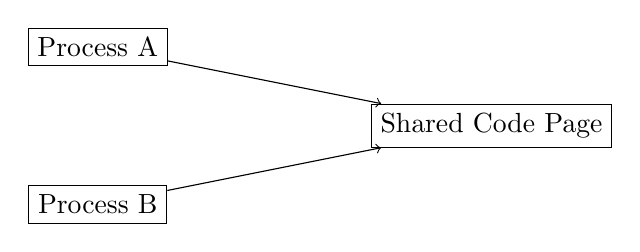
\begin{tikzpicture}

\node[draw] (p1) at (0,1) {Process A};

\node[draw] (p2) at (0,-1) {Process B};

\node[draw] (code) at (5,0) {Shared Code Page};

\draw[->] (p1)--(code);
\draw[->] (p2)--(code);

\end{tikzpicture}
\caption{Shared Pages}
\end{figure}

\section{Huge Pages}

Huge pages reduce:

\begin{itemize}
\item TLB misses
\item Page table size
\item Translation overhead
\end{itemize}

Common huge page sizes:

\begin{itemize}
\item 2 MB
\item 1 GB
\end{itemize}

\subsection{Advantages}

\begin{itemize}
\item Better performance
\item Fewer TLB entries
\end{itemize}

\section{Paging in Linux}

Linux supports:

\begin{itemize}
\item Demand paging
\item Copy-on-write
\item Huge pages
\item Transparent Huge Pages (THP)
\item Multilevel page tables
\end{itemize}

Typical x86-64 paging:

\begin{itemize}
\item PGD
\item PUD
\item PMD
\item PTE
\end{itemize}

\section{Paging in Windows}

Windows supports:

\begin{itemize}
\item Demand paging
\item Working sets
\item Large pages
\item Memory-mapped files
\end{itemize}

Features:

\begin{itemize}
\item Pagefile
\item Virtual memory manager
\item TLB optimization
\end{itemize}

\section{TLB Miss Handling}

\subsection{TLB Hit}

\begin{enumerate}
\item Lookup succeeds
\item Frame found
\item Memory accessed
\end{enumerate}

\subsection{TLB Miss}

\begin{enumerate}
\item Search page table
\item Load entry into TLB
\item Retry access
\end{enumerate}

\begin{figure}[H]
\centering
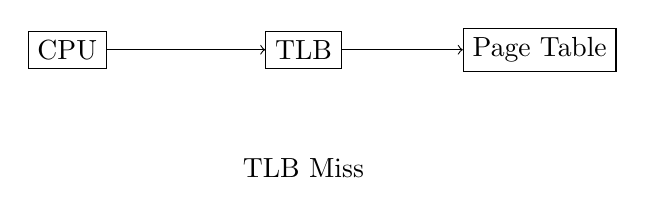
\begin{tikzpicture}

\node[draw] (cpu) at (0,0) {CPU};

\node[draw] (tlb) at (3,0) {TLB};

\node[draw] (pt) at (6,0) {Page Table};

\draw[->] (cpu)--(tlb);
\draw[->] (tlb)--(pt);

\node at (3,-1.5) {TLB Miss};

\end{tikzpicture}
\caption{TLB Miss Handling}
\end{figure}

\section{TLB Shootdown}

Occurs in multiprocessor systems.

Problem:

\begin{itemize}
\item CPU1 modifies page mapping
\item CPU2 still has stale TLB entry
\end{itemize}

Solution:

\begin{itemize}
\item Send Inter-Processor Interrupt (IPI)
\item Invalidate remote TLB entries
\end{itemize}

\begin{figure}[H]
\centering
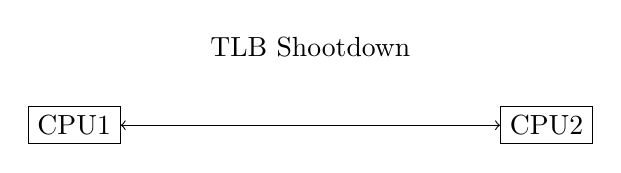
\begin{tikzpicture}

\node[draw] (cpu1) at (0,0) {CPU1};

\node[draw] (cpu2) at (6,0) {CPU2};

\draw[<->] (cpu1)--(cpu2);

\node at (3,1) {TLB Shootdown};

\end{tikzpicture}
\caption{TLB Shootdown Mechanism}
\end{figure}

\section{Interview-Focused Explanations}

\subsection{Why Paging?}

Eliminates external fragmentation.

\subsection{Why TLB?}

Reduces address translation overhead.

\subsection{Why Multilevel Paging?}

Reduces page table memory usage.

\subsection{Why Huge Pages?}

Improves TLB coverage and performance.

\subsection{Most Common Interview Formula}

\[
EMAT = h(t+m)+(1-h)(t+2m)
\]

\section{Key Takeaways}

\begin{keytakeaways}
Paging divides logical memory into pages and physical memory into frames of equal size. Address translation maps pages to frames through page tables. TLBs accelerate translation by caching page table entries. Effective Memory Access Time depends heavily on TLB hit ratio. Modern systems use multilevel, inverted, and hashed page tables to support large address spaces efficiently. Huge pages reduce translation overhead, while TLB shootdowns maintain consistency in multicore systems.
\end{keytakeaways}

\section{Interview Questions with Answers}

\begin{enumerate}
\item What is paging?\\
A memory management technique using pages and frames.

\item Why is paging used?\\
To eliminate external fragmentation.

\item What is a page?\\
Fixed-size logical memory block.

\item What is a frame?\\
Fixed-size physical memory block.

\item Relationship between page and frame size?\\
They are equal.

\item What is logical address?\\
Address generated by CPU.

\item What is physical address?\\
Actual RAM address.

\item What is address translation?\\
Logical-to-physical mapping.

\item What is a page table?\\
Maps pages to frames.

\item What is a PTE?\\
Page Table Entry.

\item What is a valid bit?\\
Indicates page presence.

\item What is a dirty bit?\\
Indicates page modification.

\item What is a reference bit?\\
Tracks recent usage.

\item What is TLB?\\
Translation Lookaside Buffer.

\item Why use TLB?\\
Speed up address translation.

\item What is TLB hit?\\
Entry found in TLB.

\item What is TLB miss?\\
Entry absent from TLB.

\item What is EMAT?\\
Effective Memory Access Time.

\item Why hierarchical paging?\\
Reduce page table size.

\item What is multilevel paging?\\
Paging using multiple page-table levels.

\item What is an inverted page table?\\
One entry per frame.

\item What is a hashed page table?\\
Hash-based virtual page lookup.

\item What are shared pages?\\
Pages mapped into multiple processes.

\item What are huge pages?\\
Large page-size mappings.

\item What is TLB shootdown?\\
Invalidating stale TLB entries across CPUs.
\end{enumerate}

\section{MCQs with Answers}

\begin{enumerate}
\item Paging eliminates:
\begin{enumerate}[label=(\alph*)]
\item Internal Fragmentation
\item External Fragmentation
\item Thrashing
\item Deadlock
\end{enumerate}
Answer: (b)

\item Physical memory is divided into:
\begin{enumerate}[label=(\alph*)]
\item Pages
\item Frames
\item Segments
\item Blocks
\end{enumerate}
Answer: (b)

\item Logical memory is divided into:
\begin{enumerate}[label=(\alph*)]
\item Frames
\item Pages
\item Chunks
\item Segments
\end{enumerate}
Answer: (b)

\item Page size equals:
\begin{enumerate}[label=(\alph*)]
\item Segment Size
\item Frame Size
\item Cache Size
\item TLB Size
\end{enumerate}
Answer: (b)

\item TLB stands for:
\begin{enumerate}[label=(\alph*)]
\item Translation Lookaside Buffer
\item Translation Link Buffer
\item Table Lookup Buffer
\item Temporary Lookup Block
\end{enumerate}
Answer: (a)

\item TLB is a:
\begin{enumerate}[label=(\alph*)]
\item Cache
\item Register
\item Disk
\item Process
\end{enumerate}
Answer: (a)

\item Address translation converts:
\begin{enumerate}[label=(\alph*)]
\item Physical to Logical
\item Logical to Physical
\item Cache to RAM
\item Virtual to Disk
\end{enumerate}
Answer: (b)

\item PTE stands for:
\begin{enumerate}[label=(\alph*)]
\item Page Table Entry
\item Physical Table Entry
\item Process Table Entry
\item Paging Translation Entry
\end{enumerate}
Answer: (a)

\item Dirty bit indicates:
\begin{enumerate}[label=(\alph*)]
\item Modified Page
\item Deleted Page
\item Free Page
\item Invalid Page
\end{enumerate}
Answer: (a)

\item Valid bit indicates:
\begin{enumerate}[label=(\alph*)]
\item Page Presence
\item Cache Presence
\item Disk Presence
\item CPU Presence
\end{enumerate}
Answer: (a)

\item TLB miss requires:
\begin{enumerate}[label=(\alph*)]
\item Page Table Lookup
\item Disk Access
\item Scheduling
\item DMA
\end{enumerate}
Answer: (a)

\item Huge pages reduce:
\begin{enumerate}[label=(\alph*)]
\item TLB Misses
\item CPU Frequency
\item Registers
\item Threads
\end{enumerate}
Answer: (a)

\item Multilevel paging reduces:
\begin{enumerate}[label=(\alph*)]
\item Page Table Memory
\item CPU Count
\item Cache
\item Processes
\end{enumerate}
Answer: (a)

\item Shared pages are commonly used for:
\begin{enumerate}[label=(\alph*)]
\item Libraries
\item Registers
\item Schedulers
\item DMA
\end{enumerate}
Answer: (a)

\item Inverted page tables contain:
\begin{enumerate}[label=(\alph*)]
\item One Entry per Frame
\item One Entry per Page
\item One Entry per Process
\item One Entry per CPU
\end{enumerate}
Answer: (a)

\item Hashed page tables use:
\begin{enumerate}[label=(\alph*)]
\item Hash Function
\item Scheduler
\item Cache
\item DMA
\end{enumerate}
Answer: (a)

\item Linux supports:
\begin{enumerate}[label=(\alph*)]
\item Demand Paging
\item Huge Pages
\item THP
\item All of the Above
\end{enumerate}
Answer: (d)

\item TLB shootdown occurs in:
\begin{enumerate}[label=(\alph*)]
\item Multiprocessors
\item Single-Core Systems
\item Embedded Devices Only
\item BIOS
\end{enumerate}
Answer: (a)

\item EMAT depends on:
\begin{enumerate}[label=(\alph*)]
\item Hit Ratio
\item Memory Time
\item TLB Time
\item All of the Above
\end{enumerate}
Answer: (d)

\item Common page size:
\begin{enumerate}[label=(\alph*)]
\item 4 KB
\item 3 KB
\item 7 KB
\item 5 KB
\end{enumerate}
Answer: (a)

\item Logical address contains:
\begin{enumerate}[label=(\alph*)]
\item Page Number
\item Offset
\item Both
\item Neither
\end{enumerate}
Answer: (c)

\item Physical address contains:
\begin{enumerate}[label=(\alph*)]
\item Frame Number
\item Offset
\item Both
\item Neither
\end{enumerate}
Answer: (c)

\item Huge pages improve:
\begin{enumerate}[label=(\alph*)]
\item Performance
\item TLB Reach
\item Translation Efficiency
\item All of the Above
\end{enumerate}
Answer: (d)

\item TLB stores:
\begin{enumerate}[label=(\alph*)]
\item Page Table Entries
\item Processes
\item Files
\item Threads
\end{enumerate}
Answer: (a)

\item Main advantage of paging:
\begin{enumerate}[label=(\alph*)]
\item Eliminates External Fragmentation
\item Eliminates Internal Fragmentation
\item Prevents Deadlock
\item Prevents Thrashing
\end{enumerate}
Answer: (a)
\end{enumerate}

\section{Revision Notes}

\begin{revisionnotes}
\item Paging divides memory into pages and frames.
\item Page size equals frame size.
\item Logical addresses contain page number and offset.
\item Physical addresses contain frame number and offset.
\item Page tables map pages to frames.
\item TLB caches page table entries.
\item EMAT depends on TLB hit ratio.
\item Hierarchical paging reduces page table overhead.
\item Multilevel paging is used in modern systems.
\item Inverted page tables use one entry per frame.
\item Hashed page tables support large virtual spaces.
\item Shared pages reduce memory consumption.
\item Huge pages improve TLB efficiency.
\item Linux supports THP and huge pages.
\item TLB shootdowns maintain consistency across CPUs.
\end{revisionnotes}

\section{Cheat Sheet}

\begin{longtable}{|p{5cm}|p{8cm}|}
\hline
Concept & Summary \\
\hline
Paging & Non-contiguous memory allocation \\
\hline
Page & Logical memory block \\
\hline
Frame & Physical memory block \\
\hline
Page Table & Maps pages to frames \\
\hline
PTE & Page Table Entry \\
\hline
TLB & Translation cache \\
\hline
TLB Hit & Entry found \\
\hline
TLB Miss & Page-table lookup required \\
\hline
EMAT & Effective Memory Access Time \\
\hline
Hierarchical Paging & Tree-structured page tables \\
\hline
Multilevel Paging & Multiple translation levels \\
\hline
Inverted Page Table & One entry per frame \\
\hline
Hashed Page Table & Hash-based lookup \\
\hline
Shared Pages & Shared mappings \\
\hline
Huge Pages & Large page sizes \\
\hline
Linux Paging & PGD/PUD/PMD/PTE \\
\hline
Windows Paging & Working-set based VM \\
\hline
TLB Shootdown & Cross-CPU invalidation \\
\hline
Need Formula & EMAT=h(t+m)+(1-h)(t+2m) \\
\hline
Interview Focus & TLB, EMAT, Multilevel Paging \\
\hline
\end{longtable}